\appendix
%\section{Appendix - Resultados} \label{section:Results}

%\subsection{IIE-Br}

%\begin{table}[htb!]
%\caption{Respostas do \gls{IBCR} ao choque de 1\% do \gls{IIE-Br}}
%\label{table:irf_IBCR_IIE}
%\vspace{0.25cm}
%\small
%\begin{tabular}{
%    >{\centering\arraybackslash}m{0.5cm}
%    >{\centering\arraybackslash}m{1.5cm}
%    >{\centering\arraybackslash}m{1.25cm}
%    >{\centering\arraybackslash}m{1.5cm}
%    >{\centering\arraybackslash}m{1.25cm}
%    >{\centering\arraybackslash}m{2.25cm}
%    >{\centering\arraybackslash}m{2.25cm}
%    >{\centering\arraybackslash}m{2.25cm}
%    }
%  \hline
% UF & \makecell{Resposta \\ Mínima} & \makecell{Mês da \\ Mínima} & \makecell{Resposta \\ Máxima} & \makecell{Mês da \\ Máxima} & \makecell{Resposta \\ Acumulada \\ Até o 3 \textordmasculine\ Mês} & \makecell{Resposta \\ Acumulada \\ Até o 12\textordmasculine\ Mês} & \makecell{Resposta \\ Acumulada \\ Até o 24\textordmasculine\ Mês} \\
%  \hline
%  
%\gls{BA} & -0.0896 & 5 & 0.0341 & 25 & -0.1873 & -0.7659 & -0.6343 \\ 
%\gls{CE} & -0.0939 & 5 & 0.0437 & 25 & -0.1813 & -0.8067 & -0.6137 \\     
%\gls{ES} & -0.1601 & 6 & -0.0031 & 25 & -0.2294 & -1.5132 & -2.1144 \\    
%\gls{GO} & -0.0436 & 4 & 0.0195 & 25 & -0.0853 & -0.3874 & -0.3775 \\    
%\gls{MG} & -0.1112 & 5 & 0.0114 & 25 & -0.1220 & -0.9237 & -1.1331 \\
%\gls{PA} & -0.0217 & 8 & 0.0229 & 1 & 0.0380 & -0.1200 & -0.1020 \\      
%\gls{PR} & -0.0927 & 6 & 0.0543 & 25 & -0.0920 & -0.7315 & -0.4800 \\     
%\gls{PE} & -0.0270 & 1 & 0.0433 & 25 & -0.0555 & -0.0429 & 0.3230 \\      
%\gls{RJ} & -0.0424 & 2 & 0.0204 & 25 & -0.0852 & -0.3899 & -0.4060 \\ 
%\gls{RS} & -0.0681 & 5 & 0.0582 & 25 & -0.0965 & -0.4821 & -0.0663 \\     
%\gls{SC} & -0.0495 & 4 & 0.0602 & 25 & -0.1194 & -0.3253 & 0.1908 \\      
%\gls{SP} & -0.0706 & 6 & 0.0473 & 25 & -0.0963 & -0.6009 & -0.4153 \\  
%
%   \hline
%\end{tabular}
%\vspace{0.25cm}
%\newline
%Fonte: Elaboração própria. \newline
%Nota: Os números da função impulso resposta estão descritos em valores absolutos.
%\end{table}

%\subsection{GEPU}

\section{Appendix - Robustez} \label{section: Robustness}

\subsection{IIE-BR}

\begin{figure}[htb!]
    \caption{Robustez - IBCR após um choque da medida de incerteza IIE-Br}
    \begin{center}
        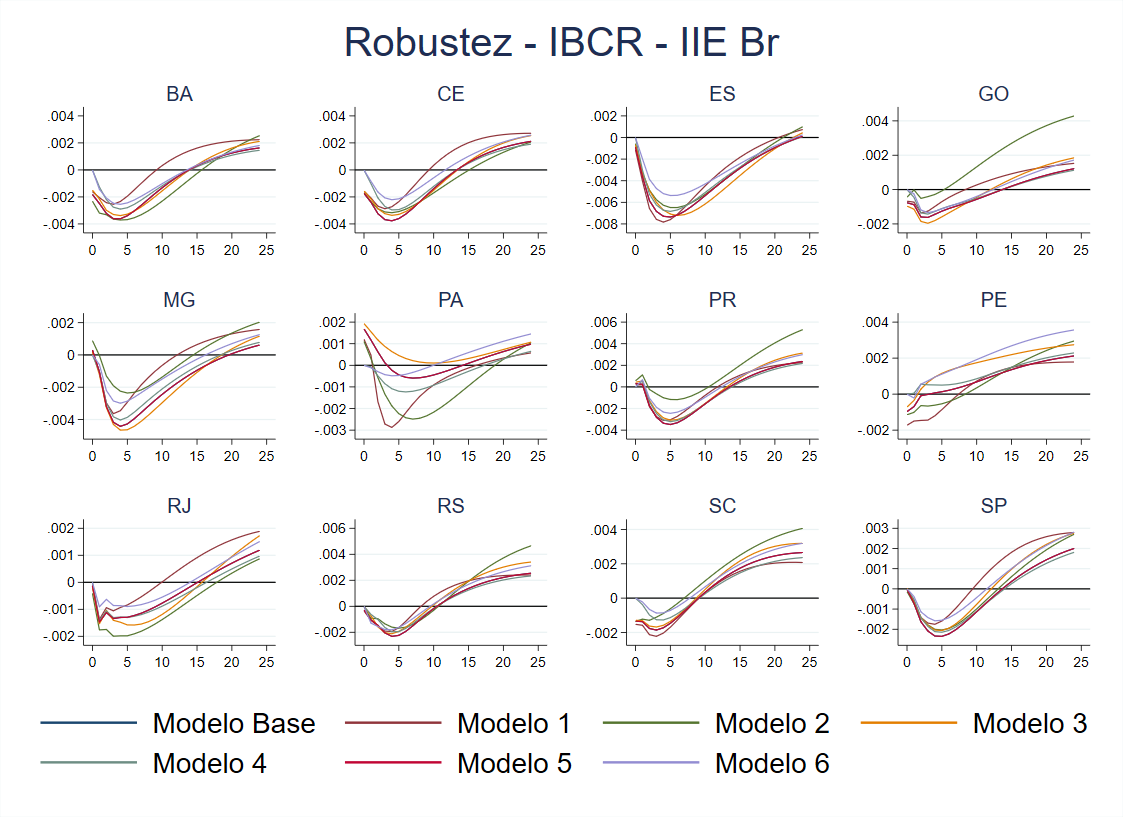
\includegraphics[width=1\linewidth]{Artigo/Fig/Robustness/IRF_IIE_IBCR_robustness.png}
    \end{center}
    \label{fig:IRF_IIE_IBCR_robustness}
Fonte: Elaboração própria. \newline
Nota: Respostas estaduais após o choque de um desvio padrão na medida de incerteza. Os números do gráfico estão descritos em valores absolutos. 
\end{figure}
\clearpage

\begin{figure}[htb!]
    \caption{Robustez - PIM após um choque da medida de incerteza IIE-Br}
    \begin{center}
        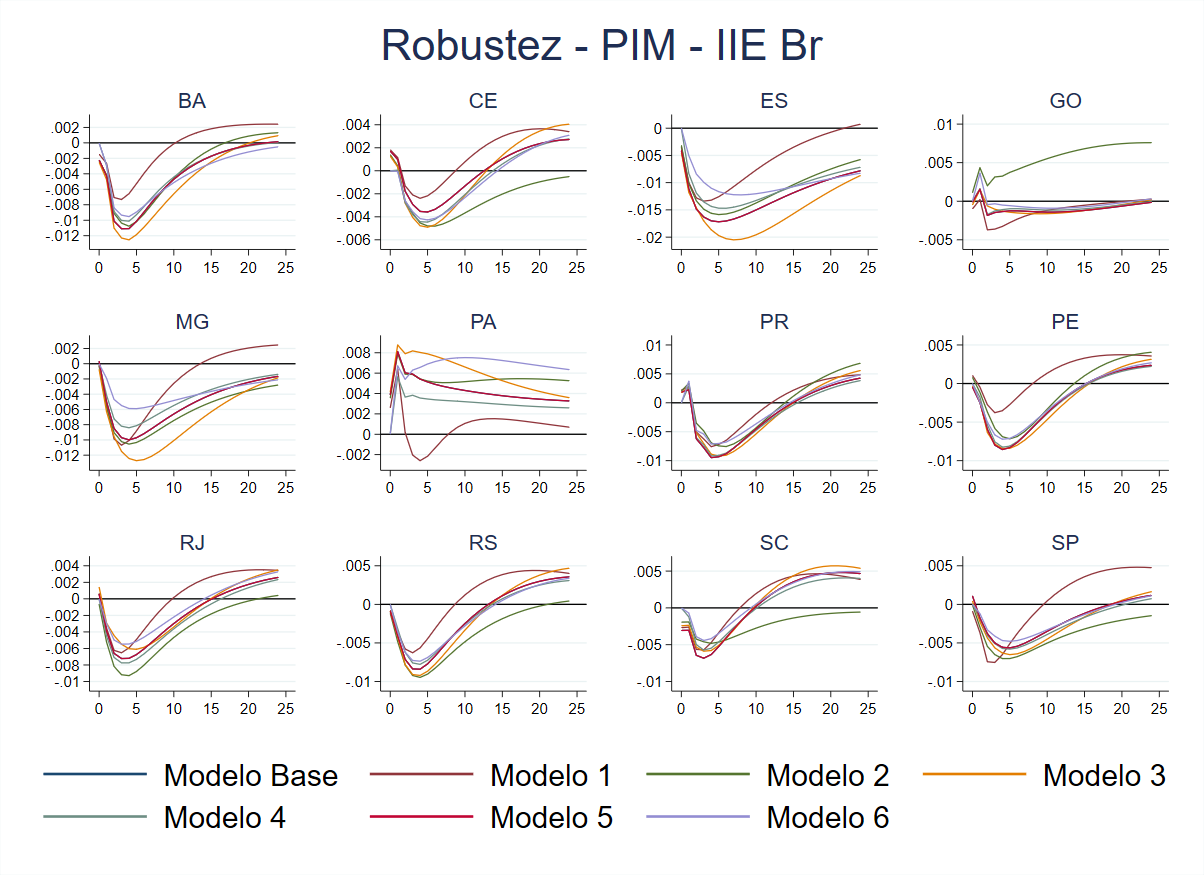
\includegraphics[width=1\linewidth]{Artigo/Fig/Robustness/IRF_IIE_PIM_robustness.png}
    \end{center}
    \label{fig:IRF_IIE_PIM_robustness}
Fonte: Elaboração própria. \newline
Nota: Respostas estaduais após o choque de um desvio padrão na medida de incerteza. Os números do gráfico estão descritos em valores absolutos.
\end{figure}
\clearpage

\subsection{EPU-BR}

\begin{figure}[htb!]
    \caption{Robustez - IBCR após um choque da medida de incerteza EPU-Br}
    \begin{center}
        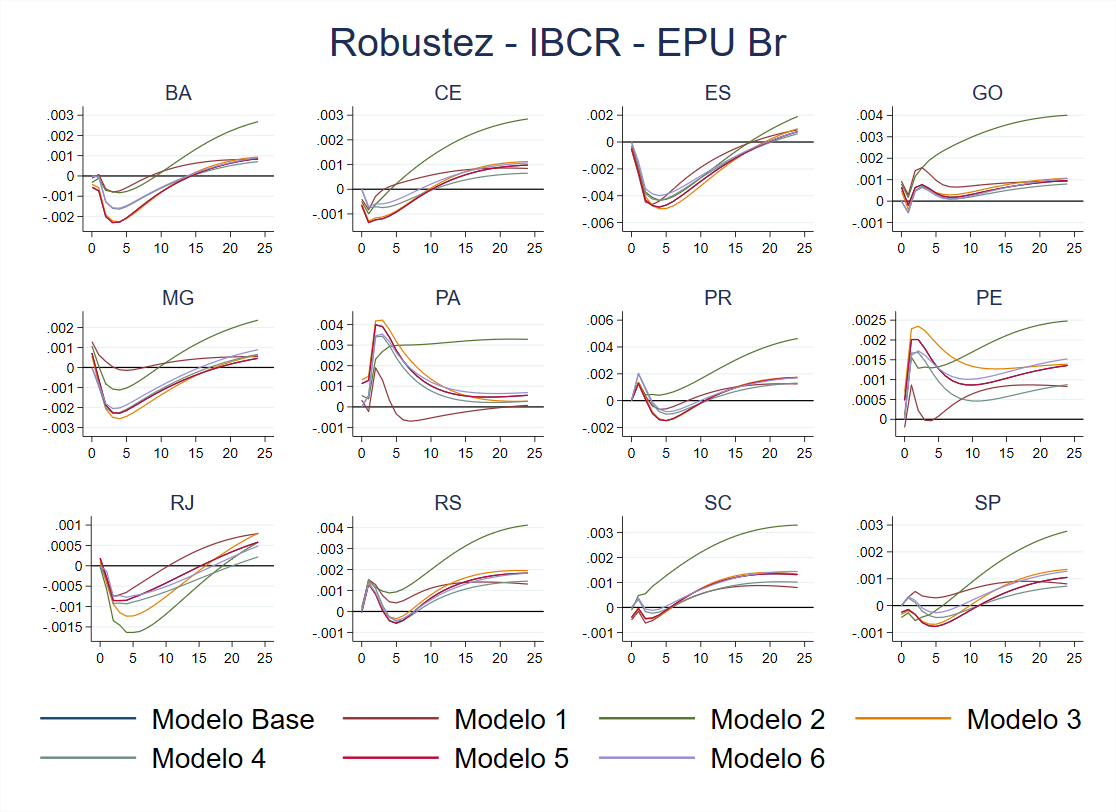
\includegraphics[width=1\linewidth]{Artigo/Fig/Robustness/IRF_EPU_IBCR_robustness.png}
    \end{center}
    \label{fig:IRF_EPU_IBCR_robustness}
Fonte: Elaboração própria. \newline
Nota: Os números da função impulso resposta estão descritos em valores absolutos.
\end{figure}
\clearpage

\begin{figure}[htb!]
    \caption{Robustez - PIM após um choque da medida de incerteza EPU-Br}
    \begin{center}
        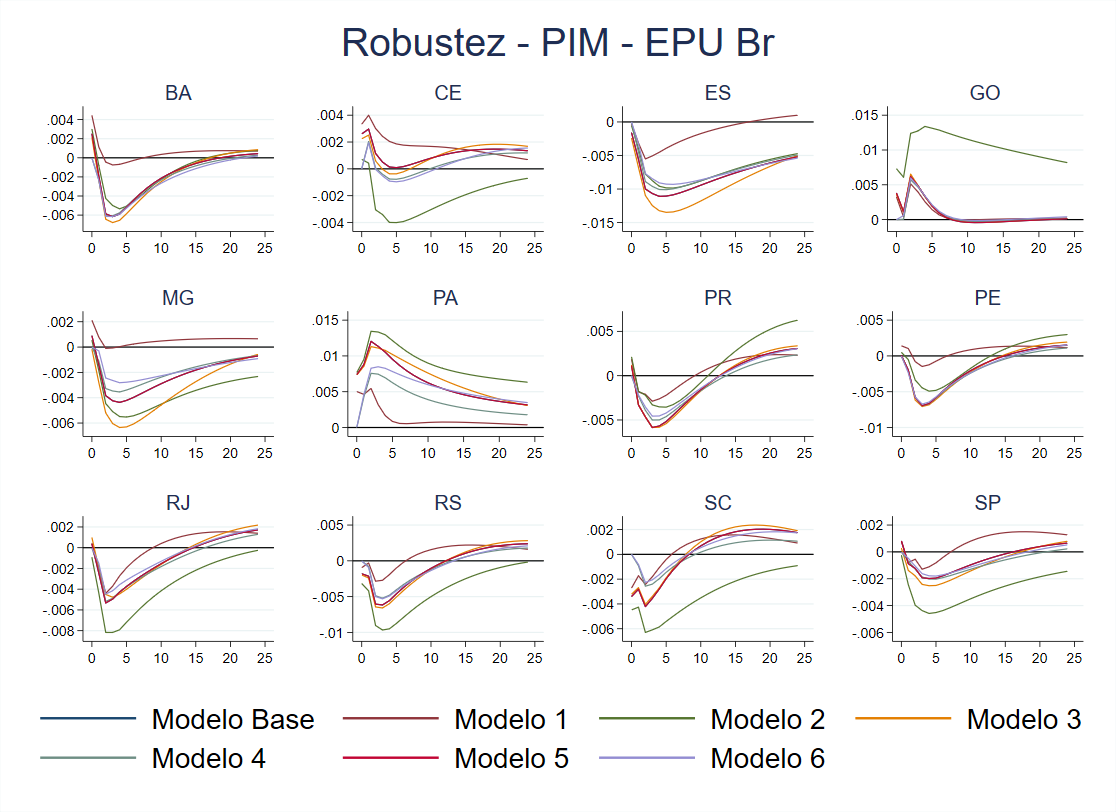
\includegraphics[width=1\linewidth]{Artigo/Fig/Robustness/IRF_EPU_PIM_robustness.png}
    \end{center}
    \label{fig:IRF_EPU_PIM_robustness}
Fonte: Elaboração própria. \newline
Nota: Os números da função impulso resposta estão descritos em valores absolutos.
\end{figure}
\clearpage

\subsection{GEPU}

\begin{figure}[htb!]
    \caption{Robustez - IBCR após um choque da medida de incerteza GEPU}
    \begin{center}
        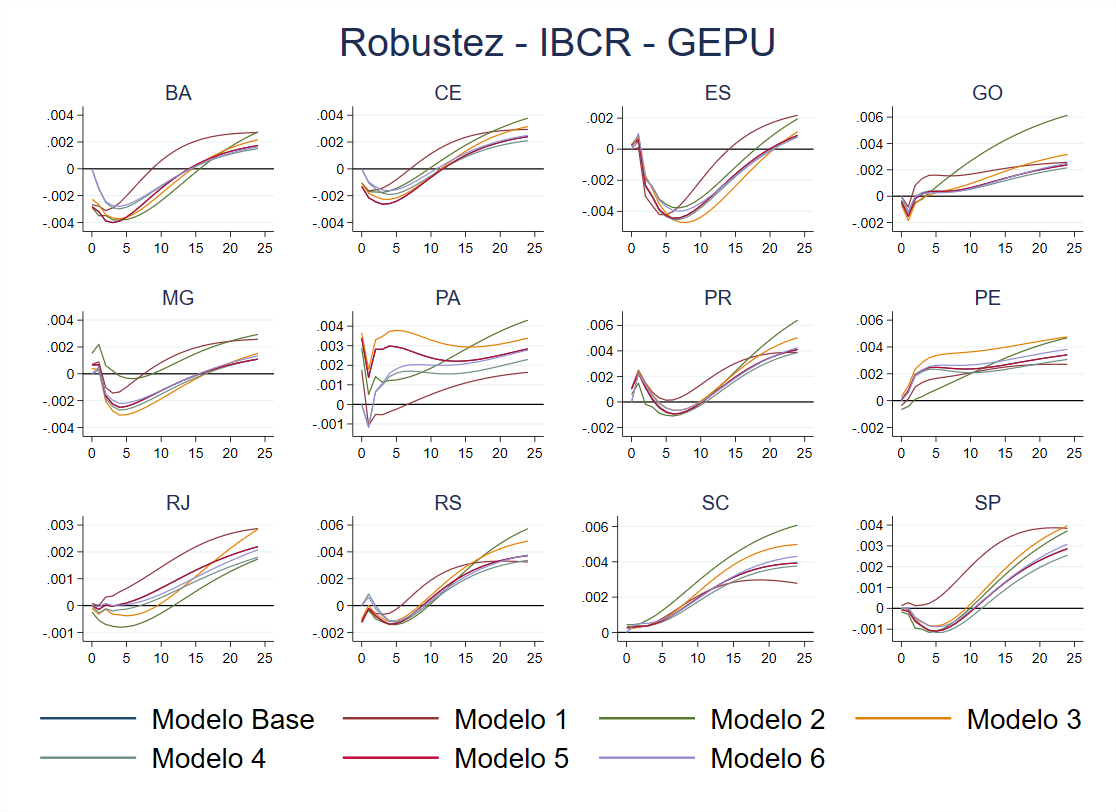
\includegraphics[width=1\linewidth]{Artigo/Fig/Robustness/IRF_GEPU_IBCR_robustness.png}
    \end{center}
    \label{fig:IRF_GEPU_IBCR_robustness}
Fonte: Elaboração própria. \newline
Nota: Os números da função impulso resposta estão descritos em valores absolutos.
\end{figure}
\clearpage

\begin{figure}[htb!]
    \caption{Robustez - PIM após um choque da medida de incerteza GEPU}
    \begin{center}
        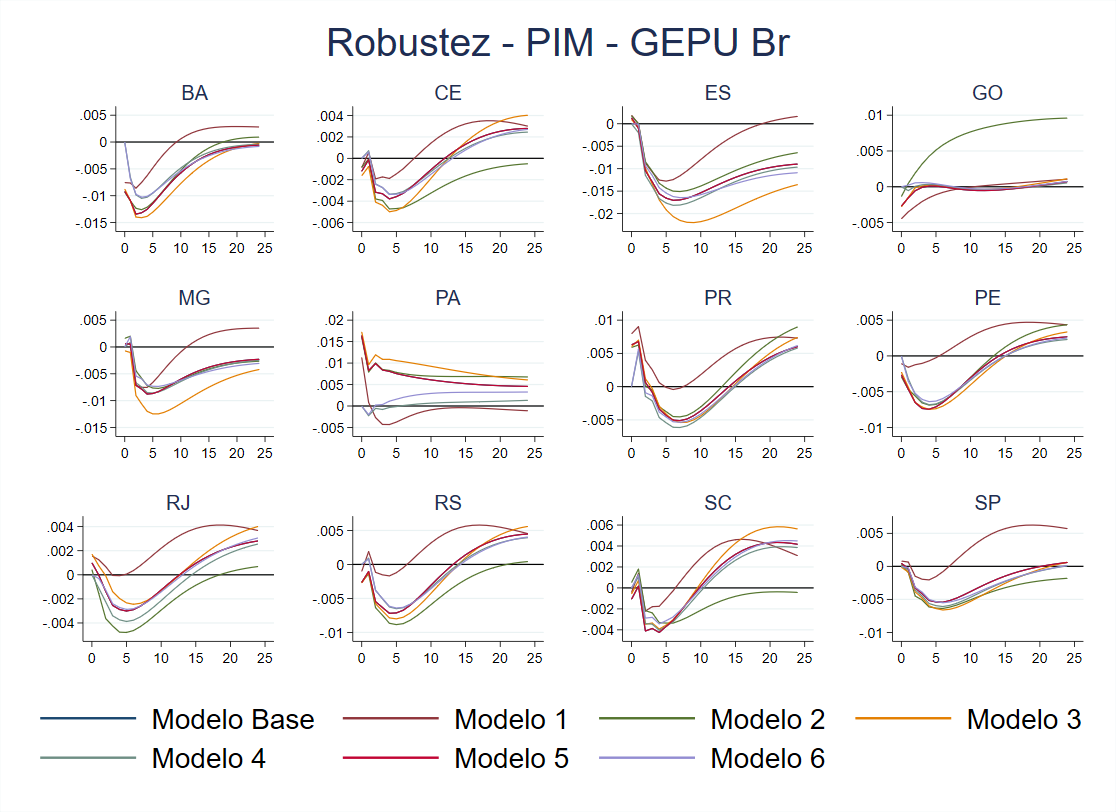
\includegraphics[width=1\linewidth]{Artigo/Fig/Robustness/IRF_GEPU_PIM_robustness.png}
    \end{center}
    \label{fig:IRF_GEPU_PIM_robustness}
Fonte: Elaboração própria. \newline
Nota: Os números da função impulso resposta estão descritos em valores absolutos.
\end{figure}
\clearpage

\section{Appendix - Cross-Section} \label{section:cross-section}

\begin{table}[htb!]
\caption{Descrição das variáveis utilizadas na regressão \textit{cross-section}}
\label{table:cross_section_labels}
\vspace{0.25cm}
\small
\begin{center}
\renewcommand{\arraystretch}{1.5}
\begin{tabular}{
    >{\raggedright\arraybackslash}m{3cm}
    |>{\raggedright\arraybackslash}m{7cm}
    |>{\centering\arraybackslash}m{2cm}
    |>{\centering\arraybackslash}m{3cm}
    %>{\centering\arraybackslash}m{1.25cm}
    %>{\centering\arraybackslash}m{2.25cm}
    %>{\centering\arraybackslash}m{2.25cm}
    %>{\centering\arraybackslash}m{2.25cm}
    }
  \hline
\textbf{Variável} & \textbf{Descrição} & \textbf{Ano(s)} & \textbf{Fonte} \\
\hline
PIB Estadual & PIB Estadual a preços de mercado (preços de 2010) & 2016 a 2019 & IPEADATA \\
\hline
\% Agropecuária & Produção agropecuária estadual dividido pelo PIB do respectivo estado & 2016 a 2019 & IPEADATA \\
\hline
\% Construção &  Produção da construção civil estadual dividido pelo PIB do respectivo estado & 2016 a 2019 & IPEADATA \\
\hline
\% Indústria Extrativa & Produção extrativa estadual dividido pelo PIB do respectivo estado & 2016 a 2019 & IPEADATA \\
\hline
\% Indústria de Transformação & Produção do setor de transformação estadual dividido pelo PIB do respectivo estado & 2016 a 2019 & IPEADATA \\
\hline
\% Serviços Financeiros & Produção de atividades financeiras, de seguros e serviços relacionados divididos pelo respectivo PIB estadual & 2016 a 2019 & IPEADATA \\
\hline
\% Serviços Públicos & Produção de serviços relacionados a administração, defesa, saúde e educação públicas e seguridade social divididos pelo respectivo PIB estadual & 2016 a 2019 & IPEADATA \\
\hline
\% Orçamento Público & Despesa corrente empenhada dividido pelo respectivo PIB estadual & 2016 a 2019 & IPEADATA \\
\hline
\% Grau de Abertura & Exportações menos importações divididos pelo respectivo PIB estadual & 2016 a 2019 & COMEXSTAT - GOV.BR \\
\hline
Densidade Demográfica & Habitante por quilômetro quadrado a nível das unidades federativas & 2022 & IBGE - Senso Demográfico 2022 - Tabela 4714 \\
\hline
\end{tabular}
\end{center}
Fonte: Elaboração própria. 
\end{table}